% Created by tikzDevice version 0.6.2-92-0ad2792 on 2013-03-23 22:57:19
% !TEX encoding = UTF-8 Unicode
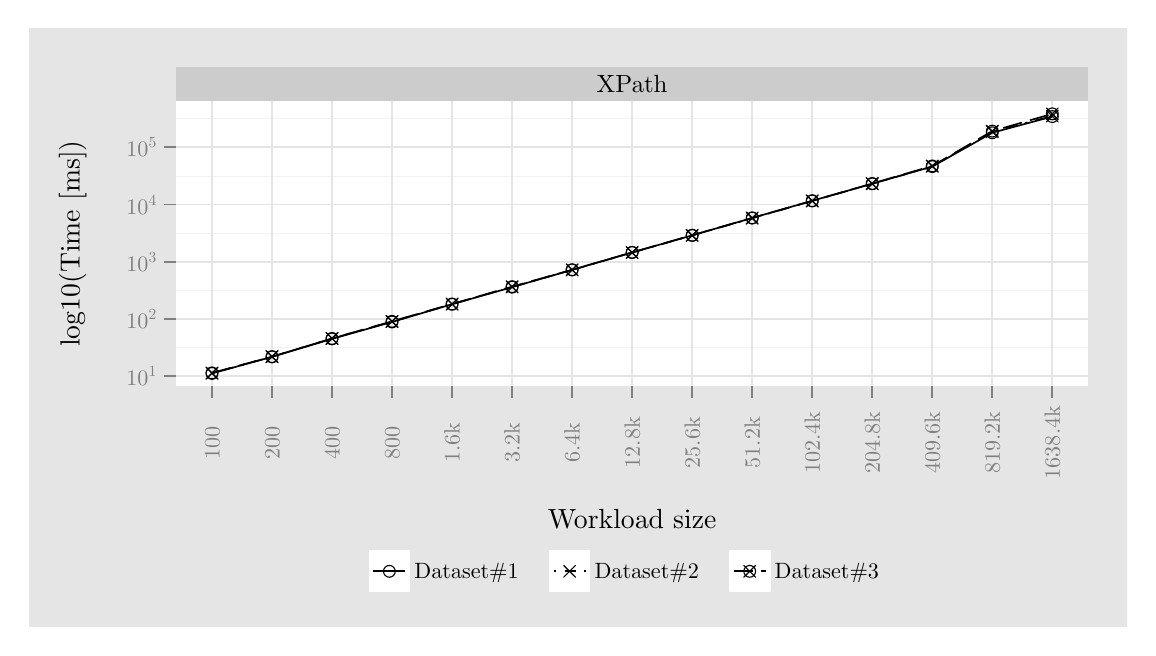
\begin{tikzpicture}[x=1pt,y=1pt]
\definecolor[named]{fillColor}{rgb}{1.00,1.00,1.00}
\path[use as bounding box,fill=fillColor,fill opacity=0.00] (0,0) rectangle (397.48,216.81);
\begin{scope}
\path[clip] (  0.00,  0.00) rectangle (397.48,216.81);
\definecolor[named]{drawColor}{rgb}{1.00,1.00,1.00}
\definecolor[named]{fillColor}{rgb}{0.90,0.90,0.90}

\path[draw=drawColor,line width= 0.6pt,line join=round,line cap=round,fill=fillColor] (  0.00,  0.00) rectangle (397.48,216.81);
\end{scope}
\begin{scope}
\path[clip] ( 53.58, 87.19) rectangle (383.26,190.36);
\definecolor[named]{fillColor}{rgb}{1.00,1.00,1.00}

\path[fill=fillColor] ( 53.58, 87.19) rectangle (383.26,190.36);
\definecolor[named]{drawColor}{rgb}{0.95,0.95,0.95}

\path[draw=drawColor,line width= 0.3pt,line join=round] ( 53.58,101.20) --
	(383.26,101.20);

\path[draw=drawColor,line width= 0.3pt,line join=round] ( 53.58,121.88) --
	(383.26,121.88);

\path[draw=drawColor,line width= 0.3pt,line join=round] ( 53.58,142.56) --
	(383.26,142.56);

\path[draw=drawColor,line width= 0.3pt,line join=round] ( 53.58,163.23) --
	(383.26,163.23);

\path[draw=drawColor,line width= 0.3pt,line join=round] ( 53.58,183.91) --
	(383.26,183.91);
\definecolor[named]{drawColor}{rgb}{0.90,0.90,0.90}

\path[draw=drawColor,line width= 0.6pt,line join=round] ( 53.58, 90.86) --
	(383.26, 90.86);

\path[draw=drawColor,line width= 0.6pt,line join=round] ( 53.58,111.54) --
	(383.26,111.54);

\path[draw=drawColor,line width= 0.6pt,line join=round] ( 53.58,132.22) --
	(383.26,132.22);

\path[draw=drawColor,line width= 0.6pt,line join=round] ( 53.58,152.89) --
	(383.26,152.89);

\path[draw=drawColor,line width= 0.6pt,line join=round] ( 53.58,173.57) --
	(383.26,173.57);

\path[draw=drawColor,line width= 0.6pt,line join=round] ( 66.60, 87.19) --
	( 66.60,190.36);

\path[draw=drawColor,line width= 0.6pt,line join=round] ( 88.29, 87.19) --
	( 88.29,190.36);

\path[draw=drawColor,line width= 0.6pt,line join=round] (109.97, 87.19) --
	(109.97,190.36);

\path[draw=drawColor,line width= 0.6pt,line join=round] (131.66, 87.19) --
	(131.66,190.36);

\path[draw=drawColor,line width= 0.6pt,line join=round] (153.35, 87.19) --
	(153.35,190.36);

\path[draw=drawColor,line width= 0.6pt,line join=round] (175.04, 87.19) --
	(175.04,190.36);

\path[draw=drawColor,line width= 0.6pt,line join=round] (196.73, 87.19) --
	(196.73,190.36);

\path[draw=drawColor,line width= 0.6pt,line join=round] (218.42, 87.19) --
	(218.42,190.36);

\path[draw=drawColor,line width= 0.6pt,line join=round] (240.11, 87.19) --
	(240.11,190.36);

\path[draw=drawColor,line width= 0.6pt,line join=round] (261.80, 87.19) --
	(261.80,190.36);

\path[draw=drawColor,line width= 0.6pt,line join=round] (283.49, 87.19) --
	(283.49,190.36);

\path[draw=drawColor,line width= 0.6pt,line join=round] (305.18, 87.19) --
	(305.18,190.36);

\path[draw=drawColor,line width= 0.6pt,line join=round] (326.87, 87.19) --
	(326.87,190.36);

\path[draw=drawColor,line width= 0.6pt,line join=round] (348.56, 87.19) --
	(348.56,190.36);

\path[draw=drawColor,line width= 0.6pt,line join=round] (370.25, 87.19) --
	(370.25,190.36);
\definecolor[named]{drawColor}{rgb}{0.00,0.00,0.00}

\path[draw=drawColor,line width= 0.6pt,line join=round] ( 66.60, 91.88) --
	( 88.29, 97.86) --
	(109.97,104.35) --
	(131.66,110.47) --
	(153.35,116.87) --
	(175.04,123.04) --
	(196.73,129.28) --
	(218.42,135.59) --
	(240.11,141.76) --
	(261.80,148.04) --
	(283.49,154.25) --
	(305.18,160.41) --
	(326.87,166.61) --
	(348.56,178.84) --
	(370.25,184.69);

\path[draw=drawColor,line width= 0.6pt,dash pattern=on 1pt off 3pt on 4pt off 3pt ,line join=round] ( 66.60, 91.91) --
	( 88.29, 97.90) --
	(109.97,104.49) --
	(131.66,110.58) --
	(153.35,116.90) --
	(175.04,123.11) --
	(196.73,129.26) --
	(218.42,135.53) --
	(240.11,141.73) --
	(261.80,147.96) --
	(283.49,154.19) --
	(305.18,160.40) --
	(326.87,166.66) --
	(348.56,179.29) --
	(370.25,184.85);

\path[draw=drawColor,line width= 0.6pt,dash pattern=on 7pt off 3pt ,line join=round] ( 66.60, 92.07) --
	( 88.29, 97.92) --
	(109.97,104.50) --
	(131.66,110.69) --
	(153.35,116.95) --
	(175.04,123.22) --
	(196.73,129.32) --
	(218.42,135.59) --
	(240.11,141.79) --
	(261.80,148.05) --
	(283.49,154.22) --
	(305.18,160.48) --
	(326.87,166.85) --
	(348.56,179.43) --
	(370.25,185.67);

\path[draw=drawColor,line width= 0.4pt,line join=round,line cap=round] ( 66.60, 91.88) circle (  2.13);

\path[draw=drawColor,line width= 0.4pt,line join=round,line cap=round] ( 88.29, 97.86) circle (  2.13);

\path[draw=drawColor,line width= 0.4pt,line join=round,line cap=round] (109.97,104.35) circle (  2.13);

\path[draw=drawColor,line width= 0.4pt,line join=round,line cap=round] (131.66,110.47) circle (  2.13);

\path[draw=drawColor,line width= 0.4pt,line join=round,line cap=round] (153.35,116.87) circle (  2.13);

\path[draw=drawColor,line width= 0.4pt,line join=round,line cap=round] (175.04,123.04) circle (  2.13);

\path[draw=drawColor,line width= 0.4pt,line join=round,line cap=round] (196.73,129.28) circle (  2.13);

\path[draw=drawColor,line width= 0.4pt,line join=round,line cap=round] (218.42,135.59) circle (  2.13);

\path[draw=drawColor,line width= 0.4pt,line join=round,line cap=round] (240.11,141.76) circle (  2.13);

\path[draw=drawColor,line width= 0.4pt,line join=round,line cap=round] (261.80,148.04) circle (  2.13);

\path[draw=drawColor,line width= 0.4pt,line join=round,line cap=round] (283.49,154.25) circle (  2.13);

\path[draw=drawColor,line width= 0.4pt,line join=round,line cap=round] (305.18,160.41) circle (  2.13);

\path[draw=drawColor,line width= 0.4pt,line join=round,line cap=round] (326.87,166.61) circle (  2.13);

\path[draw=drawColor,line width= 0.4pt,line join=round,line cap=round] (348.56,178.84) circle (  2.13);

\path[draw=drawColor,line width= 0.4pt,line join=round,line cap=round] (370.25,184.69) circle (  2.13);

\path[draw=drawColor,line width= 0.4pt,line join=round,line cap=round] ( 64.46, 89.77) -- ( 68.73, 94.04);

\path[draw=drawColor,line width= 0.4pt,line join=round,line cap=round] ( 64.46, 94.04) -- ( 68.73, 89.77);

\path[draw=drawColor,line width= 0.4pt,line join=round,line cap=round] ( 86.15, 95.77) -- ( 90.42,100.04);

\path[draw=drawColor,line width= 0.4pt,line join=round,line cap=round] ( 86.15,100.04) -- ( 90.42, 95.77);

\path[draw=drawColor,line width= 0.4pt,line join=round,line cap=round] (107.84,102.36) -- (112.11,106.63);

\path[draw=drawColor,line width= 0.4pt,line join=round,line cap=round] (107.84,106.63) -- (112.11,102.36);

\path[draw=drawColor,line width= 0.4pt,line join=round,line cap=round] (129.53,108.45) -- (133.80,112.72);

\path[draw=drawColor,line width= 0.4pt,line join=round,line cap=round] (129.53,112.72) -- (133.80,108.45);

\path[draw=drawColor,line width= 0.4pt,line join=round,line cap=round] (151.22,114.77) -- (155.49,119.04);

\path[draw=drawColor,line width= 0.4pt,line join=round,line cap=round] (151.22,119.04) -- (155.49,114.77);

\path[draw=drawColor,line width= 0.4pt,line join=round,line cap=round] (172.91,120.98) -- (177.18,125.24);

\path[draw=drawColor,line width= 0.4pt,line join=round,line cap=round] (172.91,125.24) -- (177.18,120.98);

\path[draw=drawColor,line width= 0.4pt,line join=round,line cap=round] (194.60,127.12) -- (198.87,131.39);

\path[draw=drawColor,line width= 0.4pt,line join=round,line cap=round] (194.60,131.39) -- (198.87,127.12);

\path[draw=drawColor,line width= 0.4pt,line join=round,line cap=round] (216.29,133.39) -- (220.55,137.66);

\path[draw=drawColor,line width= 0.4pt,line join=round,line cap=round] (216.29,137.66) -- (220.55,133.39);

\path[draw=drawColor,line width= 0.4pt,line join=round,line cap=round] (237.98,139.60) -- (242.24,143.87);

\path[draw=drawColor,line width= 0.4pt,line join=round,line cap=round] (237.98,143.87) -- (242.24,139.60);

\path[draw=drawColor,line width= 0.4pt,line join=round,line cap=round] (259.67,145.82) -- (263.93,150.09);

\path[draw=drawColor,line width= 0.4pt,line join=round,line cap=round] (259.67,150.09) -- (263.93,145.82);

\path[draw=drawColor,line width= 0.4pt,line join=round,line cap=round] (281.35,152.05) -- (285.62,156.32);

\path[draw=drawColor,line width= 0.4pt,line join=round,line cap=round] (281.35,156.32) -- (285.62,152.05);

\path[draw=drawColor,line width= 0.4pt,line join=round,line cap=round] (303.04,158.27) -- (307.31,162.54);

\path[draw=drawColor,line width= 0.4pt,line join=round,line cap=round] (303.04,162.54) -- (307.31,158.27);

\path[draw=drawColor,line width= 0.4pt,line join=round,line cap=round] (324.73,164.53) -- (329.00,168.79);

\path[draw=drawColor,line width= 0.4pt,line join=round,line cap=round] (324.73,168.79) -- (329.00,164.53);

\path[draw=drawColor,line width= 0.4pt,line join=round,line cap=round] (346.42,177.15) -- (350.69,181.42);

\path[draw=drawColor,line width= 0.4pt,line join=round,line cap=round] (346.42,181.42) -- (350.69,177.15);

\path[draw=drawColor,line width= 0.4pt,line join=round,line cap=round] (368.11,182.72) -- (372.38,186.98);

\path[draw=drawColor,line width= 0.4pt,line join=round,line cap=round] (368.11,186.98) -- (372.38,182.72);

\path[draw=drawColor,line width= 0.4pt,line join=round,line cap=round] ( 66.60, 92.07) circle (  2.13);

\path[draw=drawColor,line width= 0.4pt,line join=round,line cap=round] ( 64.46, 89.93) -- ( 68.73, 94.20);

\path[draw=drawColor,line width= 0.4pt,line join=round,line cap=round] ( 64.46, 94.20) -- ( 68.73, 89.93);

\path[draw=drawColor,line width= 0.4pt,line join=round,line cap=round] ( 88.29, 97.92) circle (  2.13);

\path[draw=drawColor,line width= 0.4pt,line join=round,line cap=round] ( 86.15, 95.79) -- ( 90.42,100.05);

\path[draw=drawColor,line width= 0.4pt,line join=round,line cap=round] ( 86.15,100.05) -- ( 90.42, 95.79);

\path[draw=drawColor,line width= 0.4pt,line join=round,line cap=round] (109.97,104.50) circle (  2.13);

\path[draw=drawColor,line width= 0.4pt,line join=round,line cap=round] (107.84,102.36) -- (112.11,106.63);

\path[draw=drawColor,line width= 0.4pt,line join=round,line cap=round] (107.84,106.63) -- (112.11,102.36);

\path[draw=drawColor,line width= 0.4pt,line join=round,line cap=round] (131.66,110.69) circle (  2.13);

\path[draw=drawColor,line width= 0.4pt,line join=round,line cap=round] (129.53,108.56) -- (133.80,112.83);

\path[draw=drawColor,line width= 0.4pt,line join=round,line cap=round] (129.53,112.83) -- (133.80,108.56);

\path[draw=drawColor,line width= 0.4pt,line join=round,line cap=round] (153.35,116.95) circle (  2.13);

\path[draw=drawColor,line width= 0.4pt,line join=round,line cap=round] (151.22,114.82) -- (155.49,119.09);

\path[draw=drawColor,line width= 0.4pt,line join=round,line cap=round] (151.22,119.09) -- (155.49,114.82);

\path[draw=drawColor,line width= 0.4pt,line join=round,line cap=round] (175.04,123.22) circle (  2.13);

\path[draw=drawColor,line width= 0.4pt,line join=round,line cap=round] (172.91,121.09) -- (177.18,125.35);

\path[draw=drawColor,line width= 0.4pt,line join=round,line cap=round] (172.91,125.35) -- (177.18,121.09);

\path[draw=drawColor,line width= 0.4pt,line join=round,line cap=round] (196.73,129.32) circle (  2.13);

\path[draw=drawColor,line width= 0.4pt,line join=round,line cap=round] (194.60,127.18) -- (198.87,131.45);

\path[draw=drawColor,line width= 0.4pt,line join=round,line cap=round] (194.60,131.45) -- (198.87,127.18);

\path[draw=drawColor,line width= 0.4pt,line join=round,line cap=round] (218.42,135.59) circle (  2.13);

\path[draw=drawColor,line width= 0.4pt,line join=round,line cap=round] (216.29,133.46) -- (220.55,137.72);

\path[draw=drawColor,line width= 0.4pt,line join=round,line cap=round] (216.29,137.72) -- (220.55,133.46);

\path[draw=drawColor,line width= 0.4pt,line join=round,line cap=round] (240.11,141.79) circle (  2.13);

\path[draw=drawColor,line width= 0.4pt,line join=round,line cap=round] (237.98,139.66) -- (242.24,143.92);

\path[draw=drawColor,line width= 0.4pt,line join=round,line cap=round] (237.98,143.92) -- (242.24,139.66);

\path[draw=drawColor,line width= 0.4pt,line join=round,line cap=round] (261.80,148.05) circle (  2.13);

\path[draw=drawColor,line width= 0.4pt,line join=round,line cap=round] (259.67,145.92) -- (263.93,150.19);

\path[draw=drawColor,line width= 0.4pt,line join=round,line cap=round] (259.67,150.19) -- (263.93,145.92);

\path[draw=drawColor,line width= 0.4pt,line join=round,line cap=round] (283.49,154.22) circle (  2.13);

\path[draw=drawColor,line width= 0.4pt,line join=round,line cap=round] (281.35,152.08) -- (285.62,156.35);

\path[draw=drawColor,line width= 0.4pt,line join=round,line cap=round] (281.35,156.35) -- (285.62,152.08);

\path[draw=drawColor,line width= 0.4pt,line join=round,line cap=round] (305.18,160.48) circle (  2.13);

\path[draw=drawColor,line width= 0.4pt,line join=round,line cap=round] (303.04,158.35) -- (307.31,162.62);

\path[draw=drawColor,line width= 0.4pt,line join=round,line cap=round] (303.04,162.62) -- (307.31,158.35);

\path[draw=drawColor,line width= 0.4pt,line join=round,line cap=round] (326.87,166.85) circle (  2.13);

\path[draw=drawColor,line width= 0.4pt,line join=round,line cap=round] (324.73,164.72) -- (329.00,168.99);

\path[draw=drawColor,line width= 0.4pt,line join=round,line cap=round] (324.73,168.99) -- (329.00,164.72);

\path[draw=drawColor,line width= 0.4pt,line join=round,line cap=round] (348.56,179.43) circle (  2.13);

\path[draw=drawColor,line width= 0.4pt,line join=round,line cap=round] (346.42,177.30) -- (350.69,181.57);

\path[draw=drawColor,line width= 0.4pt,line join=round,line cap=round] (346.42,181.57) -- (350.69,177.30);

\path[draw=drawColor,line width= 0.4pt,line join=round,line cap=round] (370.25,185.67) circle (  2.13);

\path[draw=drawColor,line width= 0.4pt,line join=round,line cap=round] (368.11,183.54) -- (372.38,187.81);

\path[draw=drawColor,line width= 0.4pt,line join=round,line cap=round] (368.11,187.81) -- (372.38,183.54);
\end{scope}
\begin{scope}
\path[clip] (  0.00,  0.00) rectangle (397.48,216.81);
\definecolor[named]{fillColor}{rgb}{0.80,0.80,0.80}

\path[fill=fillColor] ( 53.58,190.36) rectangle (383.26,202.58);
\definecolor[named]{drawColor}{rgb}{0.00,0.00,0.00}

\node[text=drawColor,anchor=base,inner sep=0pt, outer sep=0pt, scale=  0.90] at (218.42,193.37) {XPath};
\end{scope}
\begin{scope}
\path[clip] (  0.00,  0.00) rectangle (397.48,216.81);
\definecolor[named]{drawColor}{rgb}{0.50,0.50,0.50}

\node[text=drawColor,anchor=base west,inner sep=0pt, outer sep=0pt, scale=  0.80] at ( 35.67, 87.43) {10};

\node[text=drawColor,anchor=base west,inner sep=0pt, outer sep=0pt, scale=  0.56] at ( 43.67, 90.70) {1};

\node[text=drawColor,anchor=base west,inner sep=0pt, outer sep=0pt, scale=  0.80] at ( 35.67,108.11) {10};

\node[text=drawColor,anchor=base west,inner sep=0pt, outer sep=0pt, scale=  0.56] at ( 43.67,111.38) {2};

\node[text=drawColor,anchor=base west,inner sep=0pt, outer sep=0pt, scale=  0.80] at ( 35.67,128.79) {10};

\node[text=drawColor,anchor=base west,inner sep=0pt, outer sep=0pt, scale=  0.56] at ( 43.67,132.06) {3};

\node[text=drawColor,anchor=base west,inner sep=0pt, outer sep=0pt, scale=  0.80] at ( 35.67,149.46) {10};

\node[text=drawColor,anchor=base west,inner sep=0pt, outer sep=0pt, scale=  0.56] at ( 43.67,152.73) {4};

\node[text=drawColor,anchor=base west,inner sep=0pt, outer sep=0pt, scale=  0.80] at ( 35.67,170.14) {10};

\node[text=drawColor,anchor=base west,inner sep=0pt, outer sep=0pt, scale=  0.56] at ( 43.67,173.41) {5};
\end{scope}
\begin{scope}
\path[clip] (  0.00,  0.00) rectangle (397.48,216.81);
\definecolor[named]{drawColor}{rgb}{0.50,0.50,0.50}

\path[draw=drawColor,line width= 0.6pt,line join=round] ( 49.31, 90.86) --
	( 53.58, 90.86);

\path[draw=drawColor,line width= 0.6pt,line join=round] ( 49.31,111.54) --
	( 53.58,111.54);

\path[draw=drawColor,line width= 0.6pt,line join=round] ( 49.31,132.22) --
	( 53.58,132.22);

\path[draw=drawColor,line width= 0.6pt,line join=round] ( 49.31,152.89) --
	( 53.58,152.89);

\path[draw=drawColor,line width= 0.6pt,line join=round] ( 49.31,173.57) --
	( 53.58,173.57);
\end{scope}
\begin{scope}
\path[clip] (  0.00,  0.00) rectangle (397.48,216.81);
\definecolor[named]{drawColor}{rgb}{0.50,0.50,0.50}

\path[draw=drawColor,line width= 0.6pt,line join=round] ( 66.60, 82.92) --
	( 66.60, 87.19);

\path[draw=drawColor,line width= 0.6pt,line join=round] ( 88.29, 82.92) --
	( 88.29, 87.19);

\path[draw=drawColor,line width= 0.6pt,line join=round] (109.97, 82.92) --
	(109.97, 87.19);

\path[draw=drawColor,line width= 0.6pt,line join=round] (131.66, 82.92) --
	(131.66, 87.19);

\path[draw=drawColor,line width= 0.6pt,line join=round] (153.35, 82.92) --
	(153.35, 87.19);

\path[draw=drawColor,line width= 0.6pt,line join=round] (175.04, 82.92) --
	(175.04, 87.19);

\path[draw=drawColor,line width= 0.6pt,line join=round] (196.73, 82.92) --
	(196.73, 87.19);

\path[draw=drawColor,line width= 0.6pt,line join=round] (218.42, 82.92) --
	(218.42, 87.19);

\path[draw=drawColor,line width= 0.6pt,line join=round] (240.11, 82.92) --
	(240.11, 87.19);

\path[draw=drawColor,line width= 0.6pt,line join=round] (261.80, 82.92) --
	(261.80, 87.19);

\path[draw=drawColor,line width= 0.6pt,line join=round] (283.49, 82.92) --
	(283.49, 87.19);

\path[draw=drawColor,line width= 0.6pt,line join=round] (305.18, 82.92) --
	(305.18, 87.19);

\path[draw=drawColor,line width= 0.6pt,line join=round] (326.87, 82.92) --
	(326.87, 87.19);

\path[draw=drawColor,line width= 0.6pt,line join=round] (348.56, 82.92) --
	(348.56, 87.19);

\path[draw=drawColor,line width= 0.6pt,line join=round] (370.25, 82.92) --
	(370.25, 87.19);
\end{scope}
\begin{scope}
\path[clip] (  0.00,  0.00) rectangle (397.48,216.81);
\definecolor[named]{drawColor}{rgb}{0.50,0.50,0.50}

\node[text=drawColor,rotate= 90.00,anchor=base,inner sep=0pt, outer sep=0pt, scale=  0.80] at ( 69.35, 66.85) {100};

\node[text=drawColor,rotate= 90.00,anchor=base,inner sep=0pt, outer sep=0pt, scale=  0.80] at ( 91.04, 66.85) {200};

\node[text=drawColor,rotate= 90.00,anchor=base,inner sep=0pt, outer sep=0pt, scale=  0.80] at (112.73, 66.85) {400};

\node[text=drawColor,rotate= 90.00,anchor=base,inner sep=0pt, outer sep=0pt, scale=  0.80] at (134.42, 66.85) {800};

\node[text=drawColor,rotate= 90.00,anchor=base,inner sep=0pt, outer sep=0pt, scale=  0.80] at (156.11, 66.85) {1.6k};

\node[text=drawColor,rotate= 90.00,anchor=base,inner sep=0pt, outer sep=0pt, scale=  0.80] at (177.80, 66.85) {3.2k};

\node[text=drawColor,rotate= 90.00,anchor=base,inner sep=0pt, outer sep=0pt, scale=  0.80] at (199.49, 66.85) {6.4k};

\node[text=drawColor,rotate= 90.00,anchor=base,inner sep=0pt, outer sep=0pt, scale=  0.80] at (221.18, 66.85) {12.8k};

\node[text=drawColor,rotate= 90.00,anchor=base,inner sep=0pt, outer sep=0pt, scale=  0.80] at (242.86, 66.85) {25.6k};

\node[text=drawColor,rotate= 90.00,anchor=base,inner sep=0pt, outer sep=0pt, scale=  0.80] at (264.55, 66.85) {51.2k};

\node[text=drawColor,rotate= 90.00,anchor=base,inner sep=0pt, outer sep=0pt, scale=  0.80] at (286.24, 66.85) {102.4k};

\node[text=drawColor,rotate= 90.00,anchor=base,inner sep=0pt, outer sep=0pt, scale=  0.80] at (307.93, 66.85) {204.8k};

\node[text=drawColor,rotate= 90.00,anchor=base,inner sep=0pt, outer sep=0pt, scale=  0.80] at (329.62, 66.85) {409.6k};

\node[text=drawColor,rotate= 90.00,anchor=base,inner sep=0pt, outer sep=0pt, scale=  0.80] at (351.31, 66.85) {819.2k};

\node[text=drawColor,rotate= 90.00,anchor=base,inner sep=0pt, outer sep=0pt, scale=  0.80] at (373.00, 66.85) {1638.4k};
\end{scope}
\begin{scope}
\path[clip] (  0.00,  0.00) rectangle (397.48,216.81);
\definecolor[named]{drawColor}{rgb}{0.00,0.00,0.00}

\node[text=drawColor,anchor=base,inner sep=0pt, outer sep=0pt, scale=  1.00] at (218.42, 35.91) {Workload size};
\end{scope}
\begin{scope}
\path[clip] (  0.00,  0.00) rectangle (397.48,216.81);
\definecolor[named]{drawColor}{rgb}{0.00,0.00,0.00}

\node[text=drawColor,rotate= 90.00,anchor=base,inner sep=0pt, outer sep=0pt, scale=  1.00] at ( 18.80,138.77) {log10(Time [ms])};
\end{scope}
\begin{scope}
\path[clip] (  0.00,  0.00) rectangle (397.48,216.81);
\definecolor[named]{fillColor}{rgb}{0.90,0.90,0.90}

\path[fill=fillColor] (115.60,  8.87) rectangle (321.24, 31.86);
\end{scope}
\begin{scope}
\path[clip] (  0.00,  0.00) rectangle (397.48,216.81);
\definecolor[named]{drawColor}{rgb}{1.00,1.00,1.00}
\definecolor[named]{fillColor}{rgb}{1.00,1.00,1.00}

\path[draw=drawColor,line width= 0.6pt,line join=round,line cap=round,fill=fillColor] (123.48, 13.14) rectangle (137.93, 27.59);
\end{scope}
\begin{scope}
\path[clip] (  0.00,  0.00) rectangle (397.48,216.81);
\definecolor[named]{drawColor}{rgb}{0.00,0.00,0.00}

\path[draw=drawColor,line width= 0.6pt,line join=round] (124.92, 20.36) -- (136.49, 20.36);
\end{scope}
\begin{scope}
\path[clip] (  0.00,  0.00) rectangle (397.48,216.81);
\definecolor[named]{drawColor}{rgb}{0.00,0.00,0.00}

\path[draw=drawColor,line width= 0.4pt,line join=round,line cap=round] (130.70, 20.36) circle (  2.13);
\end{scope}
\begin{scope}
\path[clip] (  0.00,  0.00) rectangle (397.48,216.81);
\definecolor[named]{drawColor}{rgb}{1.00,1.00,1.00}
\definecolor[named]{fillColor}{rgb}{1.00,1.00,1.00}

\path[draw=drawColor,line width= 0.6pt,line join=round,line cap=round,fill=fillColor] (188.58, 13.14) rectangle (203.03, 27.59);
\end{scope}
\begin{scope}
\path[clip] (  0.00,  0.00) rectangle (397.48,216.81);
\definecolor[named]{drawColor}{rgb}{0.00,0.00,0.00}

\path[draw=drawColor,line width= 0.6pt,dash pattern=on 1pt off 3pt on 4pt off 3pt ,line join=round] (190.03, 20.36) -- (201.59, 20.36);
\end{scope}
\begin{scope}
\path[clip] (  0.00,  0.00) rectangle (397.48,216.81);
\definecolor[named]{drawColor}{rgb}{0.00,0.00,0.00}

\path[draw=drawColor,line width= 0.4pt,line join=round,line cap=round] (193.67, 18.23) -- (197.94, 22.50);

\path[draw=drawColor,line width= 0.4pt,line join=round,line cap=round] (193.67, 22.50) -- (197.94, 18.23);
\end{scope}
\begin{scope}
\path[clip] (  0.00,  0.00) rectangle (397.48,216.81);
\definecolor[named]{drawColor}{rgb}{1.00,1.00,1.00}
\definecolor[named]{fillColor}{rgb}{1.00,1.00,1.00}

\path[draw=drawColor,line width= 0.6pt,line join=round,line cap=round,fill=fillColor] (253.68, 13.14) rectangle (268.14, 27.59);
\end{scope}
\begin{scope}
\path[clip] (  0.00,  0.00) rectangle (397.48,216.81);
\definecolor[named]{drawColor}{rgb}{0.00,0.00,0.00}

\path[draw=drawColor,line width= 0.6pt,dash pattern=on 7pt off 3pt ,line join=round] (255.13, 20.36) -- (266.69, 20.36);
\end{scope}
\begin{scope}
\path[clip] (  0.00,  0.00) rectangle (397.48,216.81);
\definecolor[named]{drawColor}{rgb}{0.00,0.00,0.00}

\path[draw=drawColor,line width= 0.4pt,line join=round,line cap=round] (260.91, 20.36) circle (  2.13);

\path[draw=drawColor,line width= 0.4pt,line join=round,line cap=round] (258.77, 18.23) -- (263.04, 22.50);

\path[draw=drawColor,line width= 0.4pt,line join=round,line cap=round] (258.77, 22.50) -- (263.04, 18.23);
\end{scope}
\begin{scope}
\path[clip] (  0.00,  0.00) rectangle (397.48,216.81);
\definecolor[named]{drawColor}{rgb}{0.00,0.00,0.00}

\node[text=drawColor,anchor=base west,inner sep=0pt, outer sep=0pt, scale=  0.80] at (139.74, 17.61) {Dataset\#1 $\;\;\;$};
\end{scope}
\begin{scope}
\path[clip] (  0.00,  0.00) rectangle (397.48,216.81);
\definecolor[named]{drawColor}{rgb}{0.00,0.00,0.00}

\node[text=drawColor,anchor=base west,inner sep=0pt, outer sep=0pt, scale=  0.80] at (204.84, 17.61) {Dataset\#2 $\;\;\;$};
\end{scope}
\begin{scope}
\path[clip] (  0.00,  0.00) rectangle (397.48,216.81);
\definecolor[named]{drawColor}{rgb}{0.00,0.00,0.00}

\node[text=drawColor,anchor=base west,inner sep=0pt, outer sep=0pt, scale=  0.80] at (269.94, 17.61) {Dataset\#3 $\;\;\;$};
\end{scope}
\end{tikzpicture}
